%\documentclass[handout]{beamer}
%\usepackage{pgf,pgfpages}

\documentclass{beamer}
\usefonttheme{serif}
\usepackage[T1]{fontenc}
\usepackage{threeparttable}
\usepackage{setspace,amsfonts,amssymb,url,booktabs,tabularx,amsmath,amsthm,enumerate}
\usepackage[utopia]{mathdesign}
\usepackage{natbib,url}
\usepackage{bbm}
\usepackage{array}
\usepackage{tabu}
\usepackage{amsmath,amsfonts,amssymb,amsthm}

\theoremstyle{plain}
\newtheorem{assumption}{Assumption}

%\usepackage{beamerthemeshadow}
%Macros
\newcommand{\E}{\mathbb{E}}
\newcommand{\V}{\mathbb{V}}
\newcommand{\C}{\mathbb{C}}
\renewcommand{\r}{\mathbf{r}}
\newcommand{\XX}{\mathbf{X}}
\newcommand{\M}{\mathbf{M}}
\newcommand{\x}{\mathbf{x}}
\newcommand{\y}{\mathbf{y}}
\newcommand{\e}{\mathbf{e}}
\newcommand{\ep}{\mathbf{\epsilon}}
\newcommand{\phat}{\hat{p}}
\renewcommand{\a}{\alpha}
\renewcommand{\b}{\beta}
\renewcommand{\t}{\theta}
\newcommand{\sig}{\sum_{i=1}^N}
\newcommand{\mb}{\mathbf}
\newcommand{\bs}{\boldsymbol}
\newcommand{\sg}{\sigma}
\newcommand{\bone}{\beta_1}
\newcommand{\bzero}{\beta_0}
\newcommand{\btwo}{\beta_2}
\newcommand{\bthree}{\beta_3}
\newcommand{\bfour}{\beta_4}
\newcommand{\bzeroh}{\hat{\beta}_0}
\newcommand{\boneh}{\hat{\beta}_1}
\newcommand{\btwoh}{\hat{\beta}_2}
\newcommand{\bonet}{\tilde{\beta}_1}
\newcommand{\Ra}{\Rightarrow}
\newcommand{\ra}{\rightarrow}
\newcommand{\ital}{\textit}
\renewcommand{\bf}{\textbf}
\newcommand{\f}{\frac}
\renewcommand{\l}{\ell}
\newcommand{\h}{\hat}
\newcommand{\s}{\sum_{i=1}^N}
\newcommand{\p}{\prod_{i=1}^n}
\newcommand{\ei}{\int_{-\infty}^{\infty}}
\newcommand{\vi}{\int_{w^{*}}^{\bar{w}}}
\newcommand{\fb}{\framebox}
\newcommand{\beq}{\begin{equation}}
\newcommand{\eeq}{\end{equation}}
\newcommand{\wt}{\tilde{w}}
\newcommand{\AR}{\textup{AR}}
\newcommand{\MA}{\textup{MA}}
\newcommand*{\mybox}[1]{\framebox{#1}}
%

%\usetheme{Szeged}
\usecolortheme{beaver}
\usepackage{color}
\title{Social incentives}
\author{Anne Karing}
\date{August 17, 2015}
\begin{document}
\def\newblock{\hskip .11em plus .33em minus .07em}
\frame{\frametitle{\begin{center} Social Signaling and Prosocial Behavior \\ in Community Deworming
\end{center}}
\begin{center}
\today \\
\smallskip
Anne Karing (UC Berkeley) \\ 
\smallskip
Karim Naguib (Evidence Action)
\vspace{0.2cm}
\end{center}
}

%TO DO
%1. Change formatting of slides to either include overview OR change top, so people can see where we are.
%2. Change from small to regular sized font 
%3. Shorten the motivation. Rephrase "high take-up" to not set ourselves up for failure. 
%4. Theory, take out? Change font size of equation?
%5. Karim, distance interpretation - also should we not subtract the calendar effect to be precise?

\begin{frame}[label=slide1]
\frametitle{\large{Motivation}}
\small{
\begin{itemize}
\item According to WHO approx. 2 billion people are infected with soil-transmitted helminths (STH) worldwide. %STH refer to intestinal worms infecting humans that are transmitted through contaminated soil
\item Development burden for children and adults in many developing countries. Mild infections often are asymptomatic. More severe infections lead to abdominal pain, anemia and malnutrition.  %asymptomatic ~ go unnoticed
\item Deworming drugs are safe, no side effects for uninfected. 
\item Deworming is a public good: 
\begin{itemize}
\item Low private returns for many individuals. 
\item Most of benefits come through reduced disease transmission. 
\item Significant progress made for children through school-based deworming but remaining reservoir among adult population fosters reinfection. %slows down the potential eradication of worms
\end{itemize}
%Deworming is one of the most cost-effective ways to increase school attendance. Externalities on untreated ~ neighbors and siblings
\end{itemize}}
\end{frame}


\begin{frame}[label=slide3]
\frametitle{\large{Motivation}}
%looking at this collective action problem, ask ourselves:
%\begin{itemize}
How can we increase take-up of deworming treatment among adults within a short time in a \bf{cost-effective way}\rm? \\
\bigskip
Can we motivate adults to deworm by allowing them to \bf{signal} \rm to others that they came for treatment? 
\bigskip
\begin{itemize}
\small{
\item We can think of other behaviors that have similar public good characteristics, where we observe insufficient take-up and where formal enforcement mechanisms are very costly.}
\end{itemize}
%\end{itemize}
\end{frame}
%\small{
%More generally:
%\smallskip
%\begin{itemize}
%something as simple, cheap as that work?
%\item How does social signaling affect adults' willingness to contribute to public goods? 
%\item We can think of other behaviors with similar public good characteristics, where we observe insufficient take-up and formal enforcement mechanisms are very costly.
%cost of changing and enforcing laws or implementing at large scale material rewards
%\end{itemize}}
%\\ $\Rightarrow$ Lack of empirical evidence on social signaling. 


%We are looking at ADULT DEWORMING in the context of Kenya, Western Kenya. 
\begin{frame}[label=slide4]
\frametitle{\large{Empirical context}}
Western Kenya %worms are endemic
\begin{itemize}
 %infection prevalence is over 20$\%$. %STH infection prevalence in communities over 20%  
\item Working with Government of Kenya provided free deworming treatment to +200,000 adults in Busia, Siaya and Kakamega. %+200,000 
%Treatment was offered in two waves from October 3-14 and October 24-November 4.
\item Community Health Volunteers (CHVs) provided deworming at 144 central locations over 12 days. 
%\item Treatment was offered in two waves from October 3-14 and October 24-November 4 2016.
\item CHVs informed communities prior to deworming about the private and social benefits of deworming, the dates and location.  %key since we inform people make informed decision, knowing about the availability. further salience of public good was important to us. 
\hyperlink{slide100}{\beamerbutton{campaign script}}
\item Community deworming program first of its kind. 
%\item Kenyan Government deworms children for free in schools. School-based deworming is a well-known program.
%\item Adults can purchase deworming treatment at pharmacies and clinics for 150 KSh. %available in the market. pilot, Carol 50-200KSh
%there is no administrative data on adult deworming in Kenya. collected from baseline. 
%EXISTING KNOWLEDGE 
\item Baseline survey
\begin{itemize}
%MAIN take away the majority of people KNOWS about deworming treatment. 
\item 78$\%$ of adults know about deworming treatment, 68$\%$ have taken treatment before. %Among those, 50$\%$ said should treat every 3 months.
%Majority bought treatment at pharmacy or clinic. %Majority, 69% of 68% and 24% i.e. 16% total came for MDA at school.
%However, only about 1/3 of adults dewormed in the last 12 months. Should do every 6 months.
\item 37$\%$ reported to have dewormed in the past 12 months. %majority of those purchased treatment in the market 
%Further weak knowledge about externalities of deworming. 
\end{itemize}
\end{itemize}
\end{frame}

%EXTERNALITY KNOWLEDGE
%shooting myself in the foot with this: 31$\%$ of adults had knowledge of negative externalities. 
%said that worms can spread to others $\sim$ externality knowledge.
%Can a person sick with worms spread worms to others? 56% said no, 13% were unsure 
%ALSO asked: 
%"If you have worms, does that affect your neighbors? or relatives? health?" 28%
%"If your neighbors or relatives have worms, does that affect your health?" 25%
%stated beliefs that 70% of people would come for deworming 

\begin{frame}[label=slide6]
\frametitle{\large{Empirical context: Points-of-Treatment}}
%to illustrate the COMMUNITY LEVEL RANDOMIZATION
%in 18 subcounties
%selected clusters, with PoT and ca
%a centralized _point-of-treatment (PoT)_ at an easily identifiable location (e.g. near a church/mosque)
%catchment area of 2.5km, buffer zones 
\begin{center}
\includegraphics[width=3.3in]{map_pot}
\end{center}
\end{frame}

\begin{frame}[label=slide7]
\frametitle{\large{Theoretical framework}}
\small{
Prosocial behavior and social signaling (Benabou $\&$ Tirole 2011, 2006)}
\smallskip
\small{
Agents' preferences:
\begin{align}
U = \underbrace{(v + z - c)y}_{\text{direct benefit}}  \nonumber
\end{align}
\begin{itemize}
\small{
\item prosocial activity $y \in \{0,1\}$: to deworm or not deworm
\item $c$ cost of traveling to deworming location 
\item $z$ extrinsic motivation: consumption value of incentives
\item $v$ private and social value assigned to deworming. intrinsic motivation to 
%as a random variable
%loosely think of private or social valuation of deworming (contributing to social good)
\begin{enumerate}
\small{
\item look after your own health 
%"It is your responsibility to deworm", "It helps the community not spread worms"; "The person is improving his or her health"
\item contribute to community's health}
%"The person is disrespectful by not going for free treatment", "He or she doesn't care about his or her health"
\end{enumerate}}
\end{itemize}
$\Rightarrow$ Individuals have different types. Types are unobservable to others.} 
\end{frame}

\begin{frame}[label=slide8]
\frametitle{\large{Theoretical framework}}
%will want to think of this as static effects
\small{
Others can use your actions to draw inferences about your type.} \\
\smallskip
\small{
Agents' preferences:
\begin{align}
U = \underbrace{(v + z - c)y}_{\text{direct benefit}} + \underbrace{\mu E(v|y)}_{\text{reputational cost or benefit}}  \nonumber
\end{align}}
\small{
\begin{itemize}
\item $E(v|y)$ belief about the expectations that others will form about your type $v$ based on your action $y$ 
%second order beliefs matter here. we measured those.
%\item Individual exhibits social image concerns when her utility depends on the expectations that others form about her type, conditional on the actions that she takes 
\item $\mu$ reputational concerns, $\mu= x  \cdot \gamma$
\begin{itemize}
\item $x$ visibility or salience of $y$
%probability $y$ will be observed by others
\item $\gamma$ valuation to appear prosocial, health-conscious \\
$\Rightarrow$95$\%$ consider taking deworming treatment as praiseworthy, $69\%$ view negatively who did not take free deworming treatment.
%SAY OUT LOUD
%"The person is improving his or her health", "It is your responsibility to deworm"
%"It helps the community not to spread worms"
%There are social image/norm concerns around deworming, comparable to the use of latrines and immunization of children 
%STIGMA: "Would you praise someone for coming for free deworming at a central location?" 70% i.e. 30% would not.
%PRAISE: "Would you look down upon someone who does not come for free deworming at a central location?" 95%
\end{itemize}
\end{itemize}}
\end{frame}

\begin{frame}[label=slide9]
\frametitle{\large{Theoretical framework: Predictions}}
\small{In the absence of visibility, in equilibrium: 
\begin{align}
 %U(1) - U(0) & = v + y - c > 0  \text{ \ \ then a = 1  \ \ }    \nonumber \\
 v^{*} = c - z &  \text{ \ \ cut-off type $v^{*}$ is pinned down by direct benefits \ \ }  \nonumber  
 %separation in types according to true intrinsic motivation 
\end{align}}
\small{In presence of visibility: %should I talk about equilibrium solution, yes? 
\begin{align}
 v_r^{*} = c - z - \underbrace{\mu[E(v_r^{*}| y = 1) - E(v_r^{*}|y = 0)]}_{\text{\bf{r}\rm eputational returns: difference in the average type based on \bf{observed} \rm action}}   \nonumber 
\end{align}}
\begin{enumerate}
\item $v_r^{*}$ < $v^{*}$ individuals with lower intrinsic motivation take up deworming treatment
%as they know think that others will have information about their actions, 2nd order: what do you think they think? (accurate beliefs)
\item (signals reduce (perceived) information asymmetries in actions) %individuals believe that others have more accurate knowledge about their actions
\item increasing the visibility of signals increases reputational returns 
%there are other confounds 
\item changes in the level of take-up $v_r^{*}$ alter reputational returns $\rightarrow$ changes in cost will affect the effectiveness of signals %lead to shift in cut-off type v* and through that indirectly afffect reputational concerns 
\end{enumerate}
%someone sitting at the margin considering to deworm will now have the small extra reputational gain, being perceived as one of the good vs. bad types. visibility drives a wedge.
\end{frame}

\begin{frame}[label=slide10]
\frametitle{\large{Experimental design}}
\begin{center}
\includegraphics[width=2.5in]{signals.png}
\end{center}
Green bracelet saying "Treat worms improve the health of your community"
\end{frame}

\begin{frame}[label=slide11]
\frametitle{\large{Experimental design}}
%say that introduce visibility through incentives, which will allow individuals to form different expectations of individuals conditional on deworming or not deworming. Two signals ink and bracelet. We further introduce a material incentive, in form of a calendar that is equivalent to the consumption value of the bracelet (higher). We exogenously vary distance, to vary average take up levels exogenously to later tease if individuals are learning. Since z - ink and bracelet treatment - has also reminder, nudge effects to control for that. 
We experimentally vary the visibility, benefits and cost of deworming take-up. Individuals' utility from deworming:
\bigskip
\begin{align}
U(z) =  \underbrace{v + \textcolor{red}{z} - c}_{\text{private effect}} + \underbrace{\textcolor{red}{r(z)}}_{\text{social effect}} \nonumber   
%introduce consumption value 
\end{align}
where 
\begin{itemize}
\item \textcolor{red}{Bracelet} incentive randomized at the community level (39). 
\item Non-zero private value, high visibility as it is worn around wrist. 92$\%$ of adults say they saw people wearing these bracelets.
\end{itemize}
\end{frame}

\begin{frame}[label=slide12]
\frametitle{\large{Experimental design}}
Material reward, in form of a 2017 one-page calendar.
\begin{center}
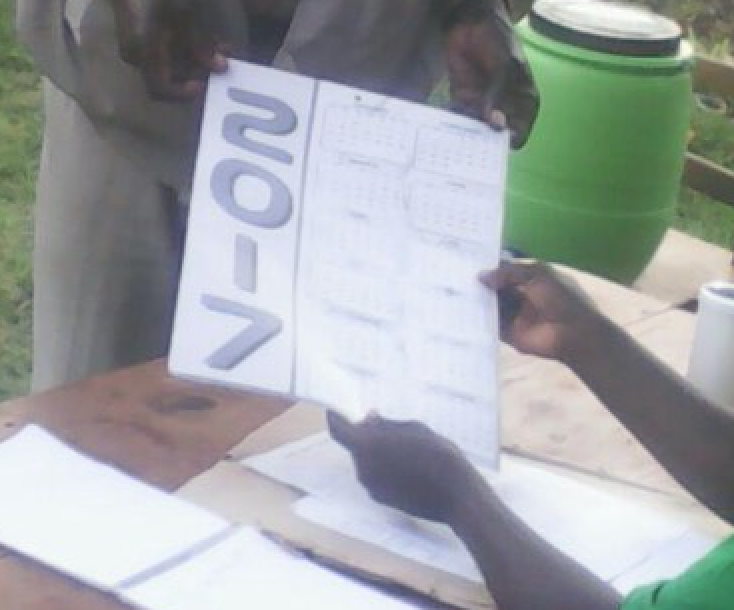
\includegraphics[width=2.5in]{calendar}
\end{center}
\end{frame}


\begin{frame}[label=slide13]
\frametitle{\large{Experimental design}}
We experimentally vary the visibility, benefits and cost of deworming take-up. Individuals' utility from deworming:
\bigskip
\begin{align}
U(z) = \underbrace{v + \textcolor{red}{z} - c}_{\text{private effect}} + \underbrace{r(z)}_{\text{social effect}}  \nonumber   
\end{align} 
where 
\begin{itemize}
\item \textcolor{red}{Calendar} incentive randomized at the community level (35).  
\item Assume $z$ of calendar is the same as that of bracelet, validated through WTP experiment. 
%control group prefer calendar over bracelets 
\hyperlink{slide101}{\beamerbutton{choice}}
\end{itemize}
\end{frame}


\begin{frame}[label=slide15]
\frametitle{\large{Experimental design}}
Indelible green ink as signal of deworming:
\begin{center}
\includegraphics[width=2in]{signal_ink}
\end{center}
%color is apolitical i.e. not associated with any party in Kenya
\end{frame}


\begin{frame}[label=slide14]
\frametitle{\large{Experimental design}}
We experimentally vary the visibility, benefits and cost of deworming take-up. Individuals' utility from deworming:
\bigskip
\begin{align}
U(z) = \underbrace{v + z - c}_{\text{private effect}} + \underbrace{\textcolor{red}{r(z)}}_{\text{social effect}}  \nonumber   
\end{align} 
where 
\begin{itemize}
\item \textcolor{red}{Ink} incentive randomized at the community level (36).
\item Has no/negative consumption value, low visibility as lasts for 3 days on skin and up to 2 weeks on nail. Used for voting.  66$\%$ of adults say they saw ink on people's finger.
\end{itemize}
%Under frequent washing 3 days, could otherwise last longer. 
%color is apolitical i.e. not associated with any party in Kenya
\end{frame}



\begin{frame}[label=slide16]
\frametitle{\large{Experimental design}\rm}
Visibility of signals: \\
\bigskip
Endline survey, conducted 3-14 days after deworming ended %asking people that were given the ink or bracelet when coming for deworming.
\smallskip
%Have you seen this ink on people's finger? Have you seen this bracelet on people's wrist?
\begin{itemize}
\item Ink: 66$\%$ of adults say they saw ink on people's finger. 15$\%$ of adults that came for deworming had ink on their fingers.
\smallskip
\item Bracelet: 92$\%$ of adults say they saw people wearing these bracelets. 47$\%$ of adults that came for deworming wore the bracelet on their wrist. 
%81$\%$ had the bracelet in their possession. 
\end{itemize}
%We need to adjust for the fact that more people came for treatment in the bracelet clusters. \item Calendar 74.86$\%$ saw calendar, among those that did not come 48.86$\%$ saw calendar.
\smallskip
%\item Retention
%\small{
%\begin{itemize}
%\item Ink: 15$\%$ of adults that came for deworming had ink on their fingers. %when visited at endline
%\item Bracelet: 47$\%$ of adults that came for deworming wore the bracelet on their wrist. 81$\%$ had the bracelet in their %possession. 
%\end{itemize}} 
\end{frame}

\begin{frame}[label=slide108]
\frametitle{\large{Empirical implementation: community sensitization}} 
\begin{center}

\includegraphics[width=2.2in]{flyer_bracelet.png}
\end{center}
\end{frame}

%show you what take-up levels broadly looked like \small{N = 2,213}
%FIRST I am going to show you what take up levels broadly look like. 
%This goes contrary to beliefs that individuals had at baseline where reported believed take up was 60%. 
\begin{frame}[label=slide17]
\frametitle{\large{Results}}
\begin{center}
\includegraphics[width=4in]{static_level_smsctrl}
\end{center}
\end{frame}

%Next I am showing you reported estimated marginal effects from the logit model, where we estimate differences in the take-up probability switching different incentive, distance, SMS treatments on or off  
%\small{N = 30,459} These will look slightly different since we are switching samples here. For IRB reasons we were only allowed to name match for a reduced sample. 
\begin{frame}[label=slide06]
\frametitle{\large{Results}}
\begin{center}
\includegraphics[width=4.4in]{static_ate_smsctrl}
\end{center}
\end{frame}
%just say here that we observe large positive effects for bracelets, shifting take-up from 36% to 44% by 23% increase in take-up

%\item Decompose bracelet effect (8.4pp) into: 
%\begin{enumerate}
%\item Consumption effect: 2.7pp 
%\item Social effect: 5.7pp $\rightarrow$ 16$\%$ (23$\%$) increase in deworming

%IN THE FOLLOWING I WILL TAKE TWO APPROACHES THAT SUGGEST THAT WHAT WE OBSERVED IS DUE TO SIGNALING and NOT SOME FORM OF OTHER SOCIAL INFLUENCE
%FIRST APPROACH
\begin{frame}[label=slide18]
\frametitle{\large{Experimental design: SMS reminders/social information}}
\small{
%main confound in pinning down signaling
As we introduce signals, individuals can observe others' decision to deworm or not deworm. Signals could \it{also} \rm work through:
\begin{itemize}
\item Updating beliefs about the benefits of deworming
\item Herding 
%\item Social consumption value in bracelets $z$ Fad
%\hyperlink{slide101}{\beamerbutton{D1}}
\item Increasing the salience of deworming and acting as reminder 
\end{itemize}}
Identify social image concerns, by controlling for salience/reminder and social learning effects through SMS treatment. 
\begin{itemize}
\item A random subset of adults was sent SMS reminders:
%that also informed them about deworming take-up in their community. 
\begin{itemize}
\item Free deworming now at [Central Location]. [No/few/almost half/half/more than half/almost all/all] of your village came, that is X in 10 adults.
\end{itemize}
\item SMS were sent the day before deworming started, on day 2, 4, 6, 8 and 10 of deworming treatment.
%randomly selected households
%randomly selected among phone owners in each of 144 clusters, recruited and people could unsubscribe from text any time. 
%25 selected in ink/bracelet/calendar, 15 in control 
%about 2/3 of population own a phone!
\end{itemize}
\end{frame}

\begin{frame}[label=slide21]
\frametitle{\large{Results}}
%\small{N = 2,358}
\begin{center}
\includegraphics[width=4.4in]{static_ate_all}
\end{center}
\hyperlink{slide102}{\beamerbutton{take-up levels}}
\end{frame}
%${-}$ 35$\%$. 
%ATEs remain constant i.e. even if I saturate you with reminders and provide you information about deworming in your community, you still respond to bracelet. No substitution, i.e. if primarily worked as reminder/salience.

\begin{frame}[label=slide22]
\frametitle{\large{Experimental design}}
We experimentally vary the visibility, benefits and cost of deworming take-up. Individuals' utility from deworming:
\bigskip
%second signal
\begin{align}
U_{i}(z,d) = \underbrace{v + z_i - c_i(\textcolor{red}{d})}_{\text{private effect}} + \underbrace{r(z,\textcolor{red}{d})}_{\text{social effect}}  \nonumber   
\end{align}
where 
\begin{itemize}
\item \textcolor{red}{Close, far} distance to treatment location, randomized at the community level (72/72).  \hyperlink{slide103}{\beamerbutton{distance random}}
\item Randomized the cost of deworming and shifted $v^{*}$. %the marginal person considering taking up deworming. as shown in previous framework
\end{itemize}
\end{frame}
%shifted distance by average of 1km extra to walk

%Distance cost had large effect on deworming take-up, reducing it from 44% to 28% - a reduction of 35% in take-up.
\begin{frame}[label=slide24]
\frametitle{\large{Results}}
\begin{center}
\includegraphics[width=4.2in]{static_level_smsctrl_dist}
\end{center}
\end{frame}

\begin{frame}[label=slide25]
\frametitle{\large{Results}}
\begin{center}
\includegraphics[width=4.4in]{static_ate_smsctrl_dist}
\end{center}
\end{frame}
%we can't reject that these are not different 

\begin{frame}[label=slide26]
\frametitle{\large{Results}}
\begin{center}
\includegraphics[width=4.4in]{with_calendar}
\end{center}
\end{frame}

%for Karim for later exp_diagram.png

\begin{frame}[label=slide26]
\frametitle{\large{Conclusion}}
\begin{enumerate}
\item Social signal significantly increase deworming take-up. 3 times the effect of small material reward.
\item Visibility and trust are key for signals to be effective. 
\item Small increases in travel cost lead to large drop in demand. Signals have large(r) effects, compensating for drop in demand. %Optimal location of treatment points
\bigskip
\item SMS reminders/recruitment visits have....
\end{enumerate}
\end{frame}



%tried to carry over same message as from school based deworming in terms of everyone should do this 
\begin{frame}[label=slide100]
\frametitle{\large{Experimental design}} 
\begin{center}
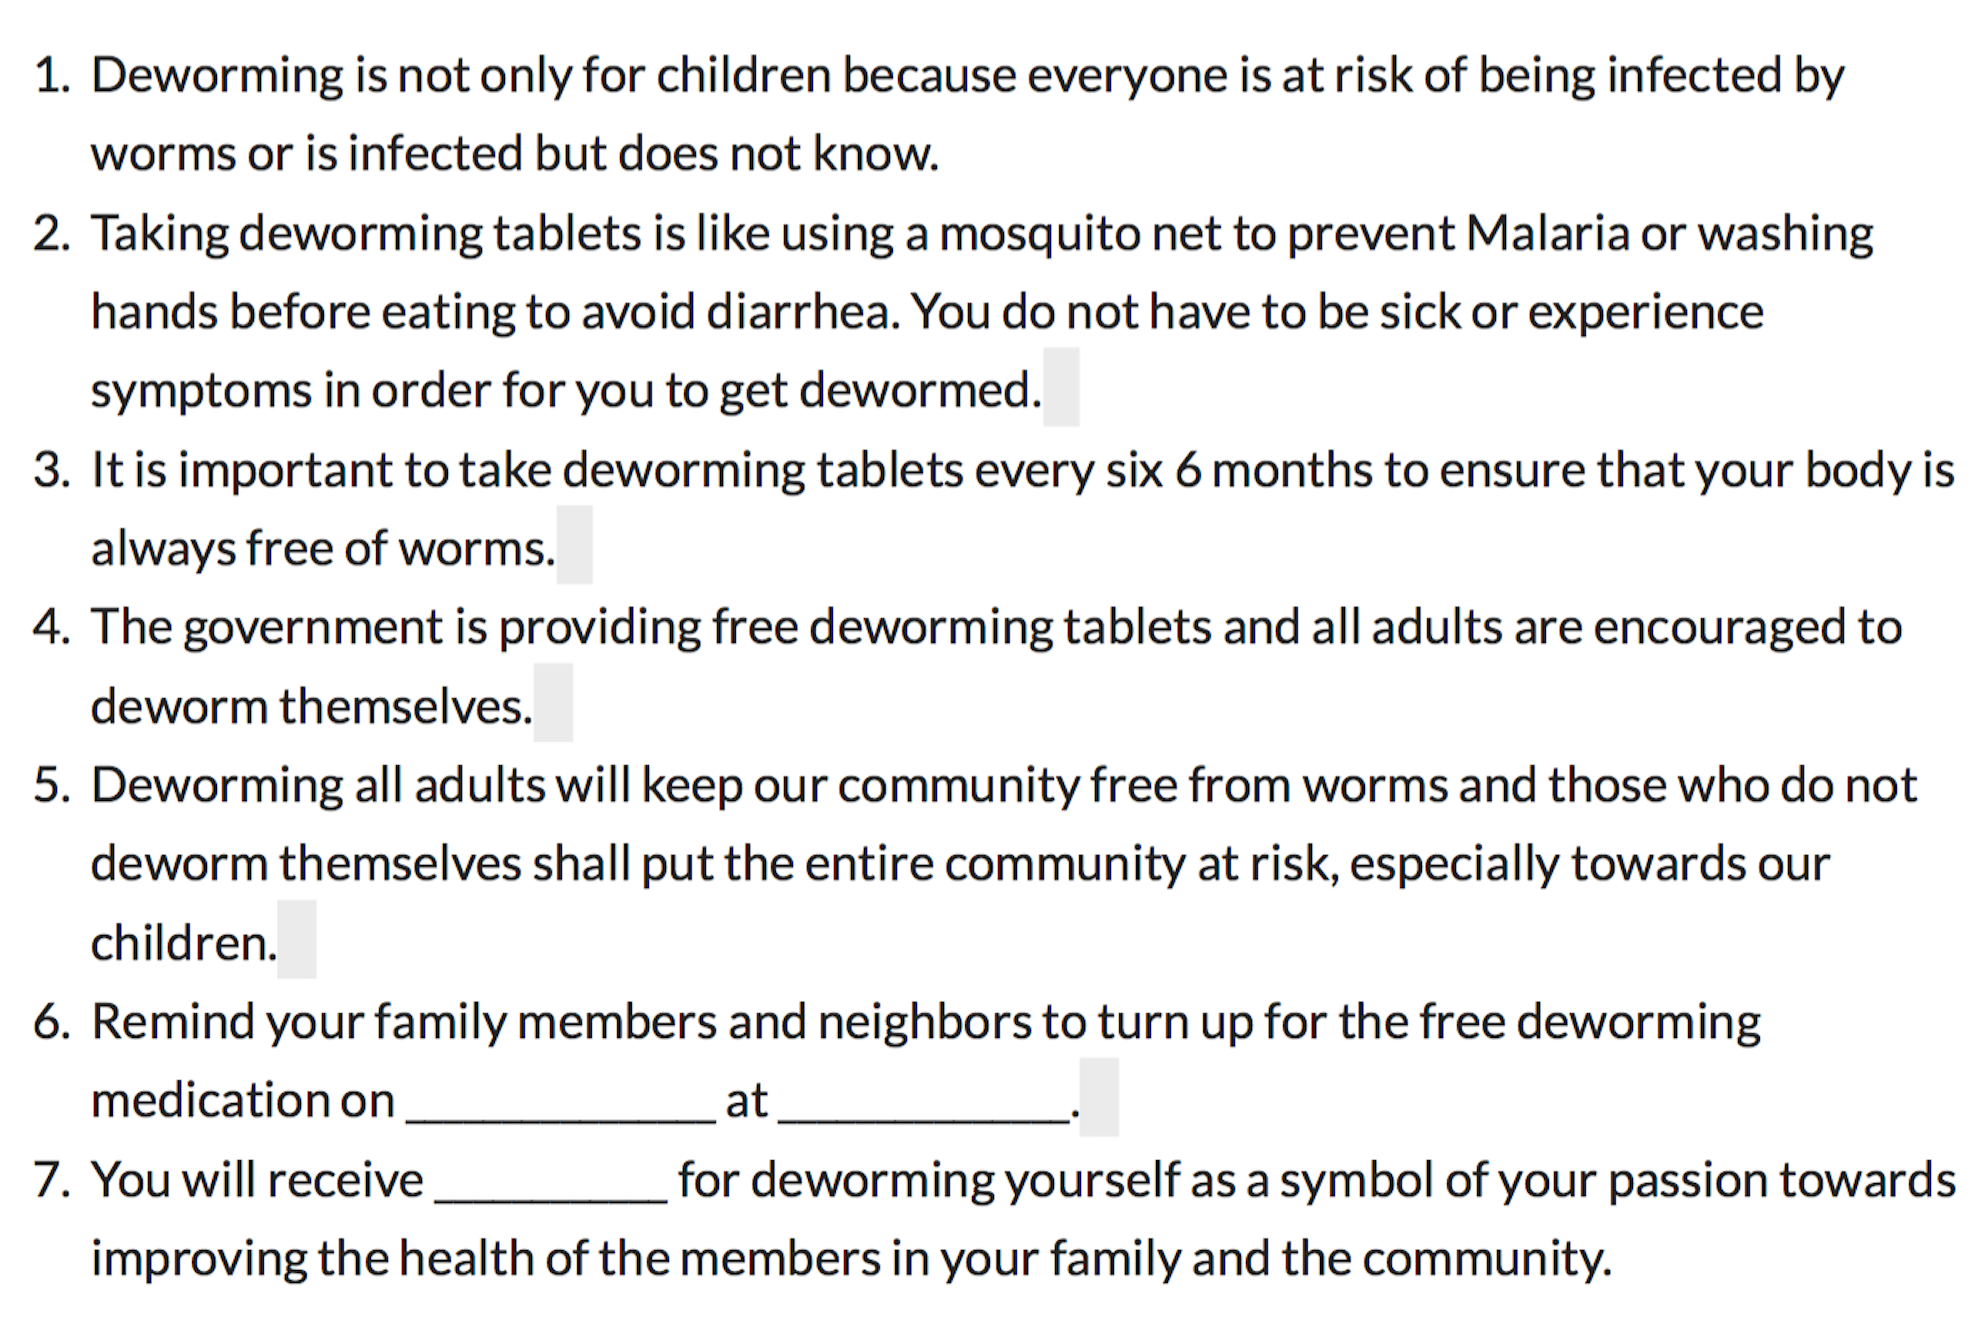
\includegraphics[width=4.4in]{sensitization}
\end{center}
\hyperlink{slide5}{\beamerbutton{context}}  
\end{frame}
%80$\%$ of respondents say they were visited by a CHV about deworming. 69$\%$ report to have received a flyer. 
%81$\%$ of respondents say that treatment was available for 10-14 days and 82$\%$ knew the correct start date.



\begin{frame}[label=slide101]
\frametitle{\large{Private value calendar vs. bracelet}}
Choice experiment in control group.
\smallskip
\begin{itemize}
\item Offered respondents a reward for completing the survey, choosing between the calendar and bracelet. 
\begin{itemize}
\item \large{75$\%$ chose calendar, 23$\%$ chose the bracelet and 2$\%$ wanted neither.}
\end{itemize}
\smallskip
\item Offered respondents to exchange their first choice (e.g. calendar) for the not chosen item (e.g. bracelet), plus a randomly assigned KSh value (between 0 to 100 KSh/USD 1)
\item On average, individuals value the calendar between 42-53 KSh more than the bracelet.
%heterogeneity over counties
%(market value calendar 31 KSh).
\end{itemize}
\smallskip
$\Rightarrow$ \large{Calendar preferred to bracelet.}
%no social utility, fad for bracelet: gave same choice to bracelet 21% chose bracelet, 78% chose the calendar. 
%we are collecting WTP data, where we get a precise estimate of the utility difference between the 2 items in terms of KSh
\hyperlink{slide13}{\beamerbutton{design}}  
\end{frame}


\begin{frame}[label=slide102]
\frametitle{\large{Results}}
\begin{center}
\includegraphics[width=4.4in]{static_level_all}
\end{center}
\hyperlink{slide21}{\beamerbutton{results}} 
\end{frame}

\begin{frame}[label=slide103]
\frametitle{\large{Experimental design}}
%\small{We experimentally vary the cost of deworming take-up...}
\begin{center}
\includegraphics[width=4.4in]{distancerandom}
\end{center}
\hyperlink{slide22}{\beamerbutton{design}} 
\end{frame}

\begin{frame}[label=slide104]
\frametitle{\large{Results}}
\begin{center}
\includegraphics[width=3.6in]{dyn_daily_all.png}
\end{center}
\end{frame}

\begin{frame}[label=slide105]
\frametitle{\large{Results}}
\begin{center}
\includegraphics[width=4.2in]{dyn_daily_all_dist.png}
\end{center}
\end{frame}

\begin{frame}[label=slide106]
\frametitle{\large{Empirical implementation: community sensitization}}
\begin{center}

\includegraphics[width=2in]{flyer_ink.png}
\end{center}
\end{frame}

\begin{frame}[label=slide107]
\frametitle{\large{Empirical implementation: community sensitization}}
\begin{center}

\includegraphics[width=2in]{flyer_calendar.png}
\end{center}
\end{frame}






\end{document}





